
\newpage
\subsection{Axis encoding} % relevance
\label{sec:axis_encoding}

\textbf{Motivation.} Looking back at the networks generated by \featureset{All} in baseline runs, the learned weigths of most neurons in the feature transformer layer (L1) are related with the movement pattern of the pieces. Let's take the example in Figure \ref{fig:rook_weights}, which depicts the \featureset{Square} part of the features where the role is \symrook\ Rook.

\begin{figure}[h]
\centering
\subfloat[\centering $\white$ White]{{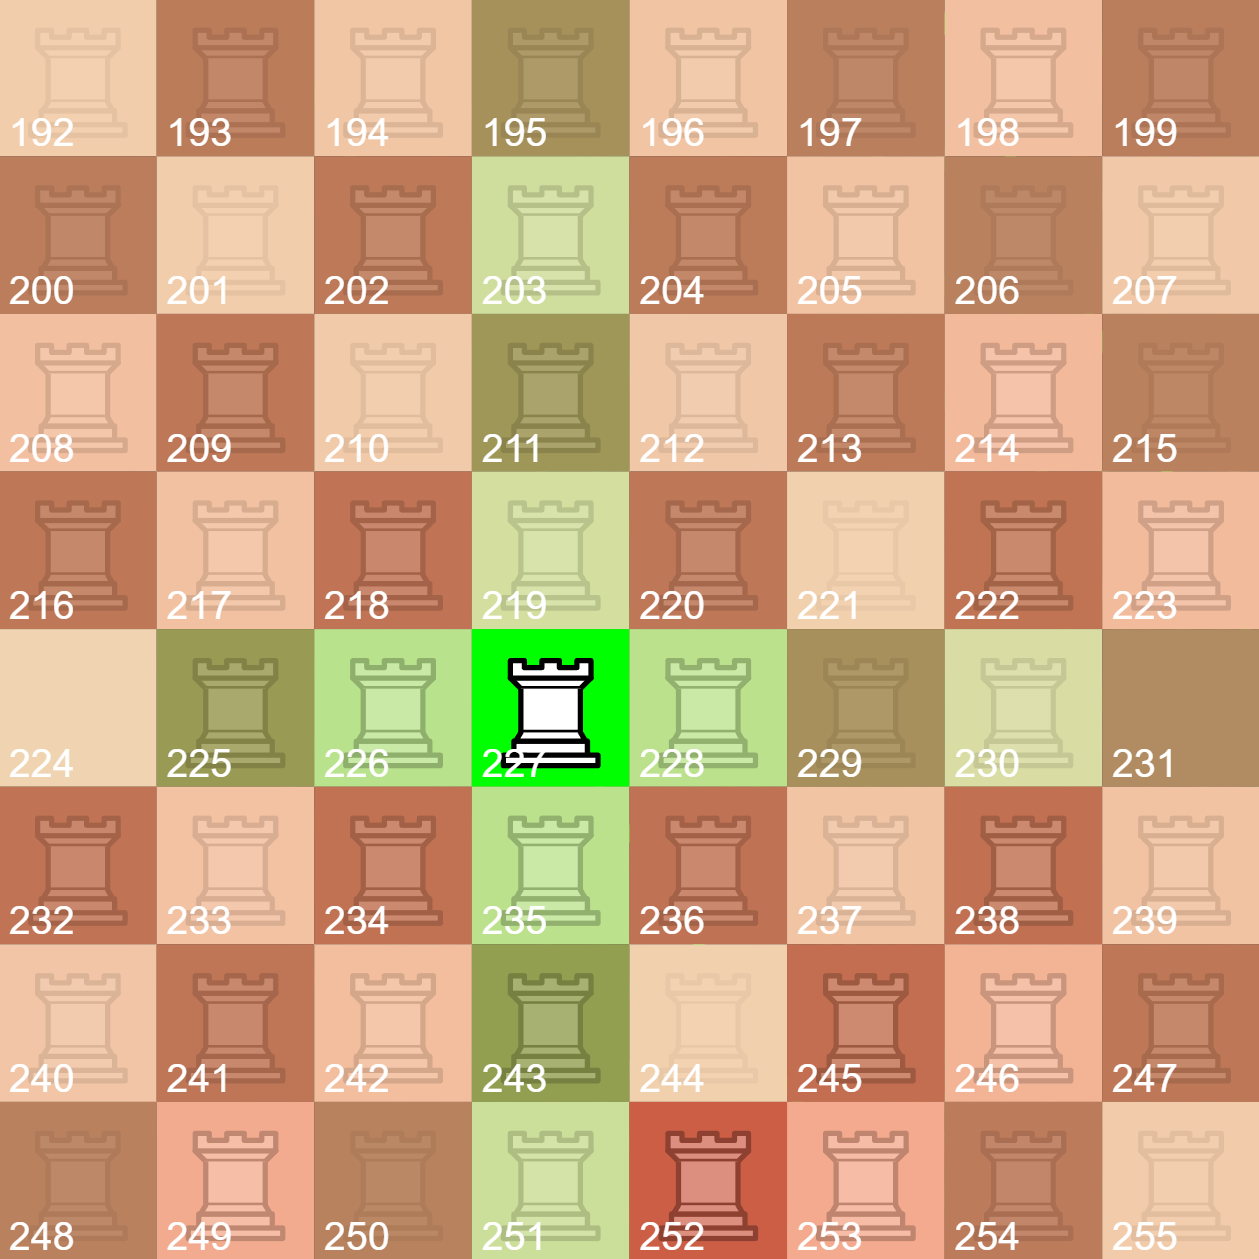
\includegraphics[width=7cm]{../assets/results/piece_weights/white_rook_weights.png} }}%
\qquad
\subfloat[\centering $\black$ Black]{{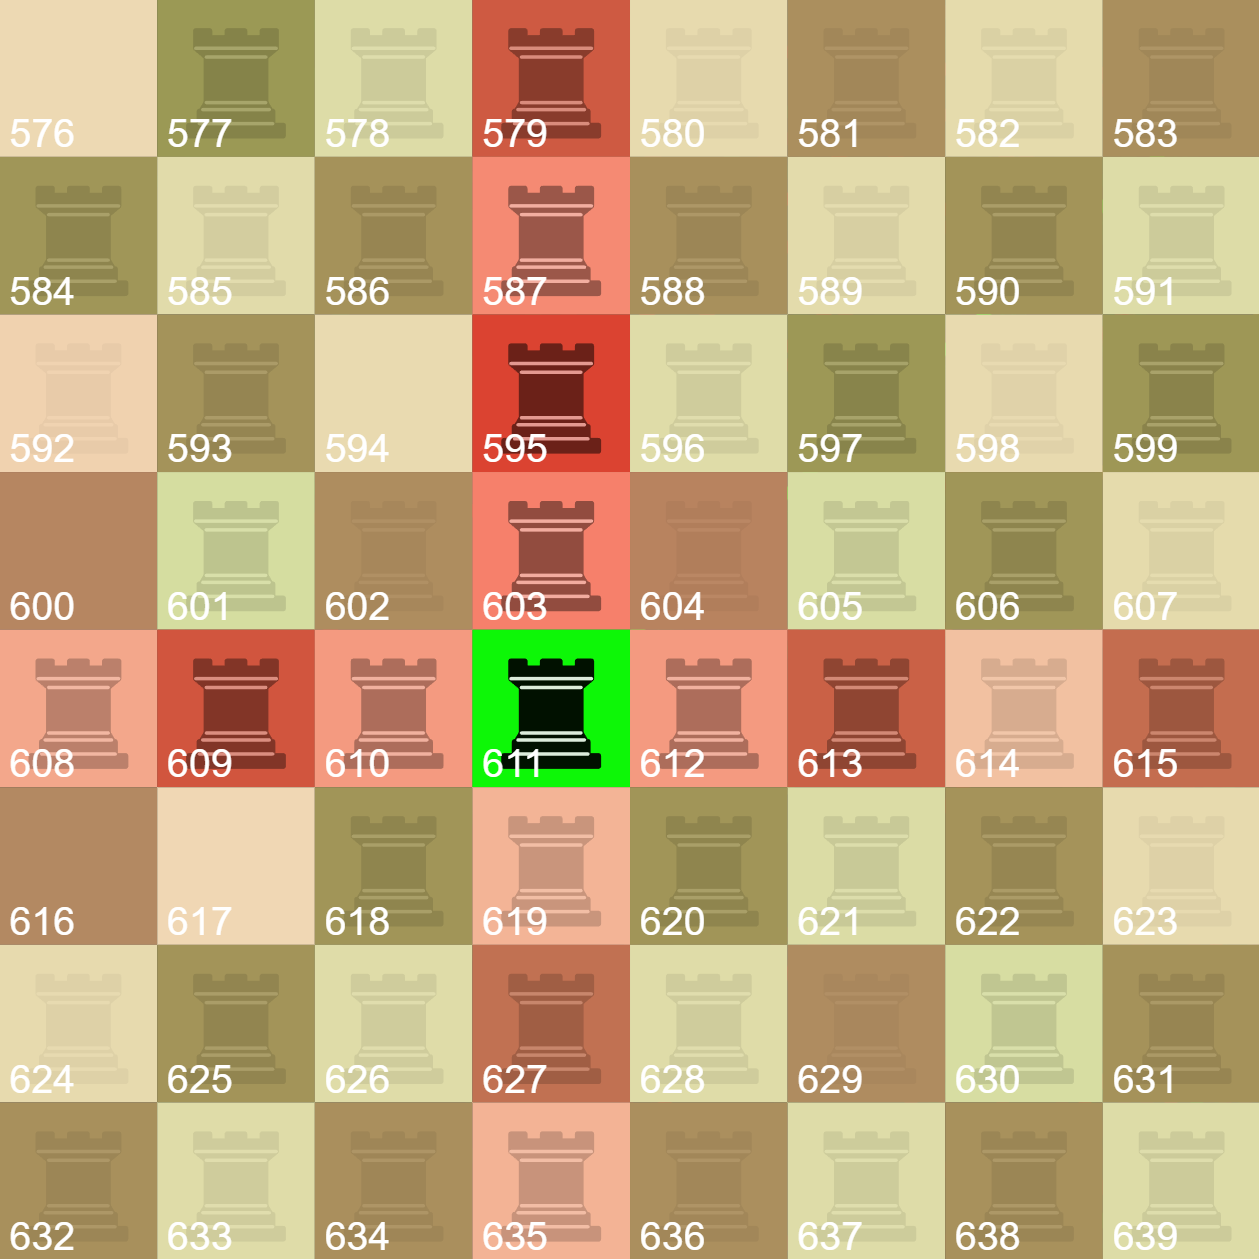
\includegraphics[width=7cm]{../assets/results/piece_weights/black_rook_weights.png} }}%
\caption{Weights of \textbf{a neuron} in the L1 layer, which are connected to features in \featureset{All} where the role is $\rook$ Rook. The intensity represents the weight value, and the color represents the sign (although not relevant).}
\label{fig:rook_weights}
\end{figure}

This particular neuron learned to recognize the presence of a rook, affected by the pattern of another potential rook in the same file or rank. Doing so, it had to relate one feature for every potential square where a rook could be for that specific center location, which restrains the network from learning more complex patterns and it is harder to train, because you need more samples to account for all possible combinations.

What if we add a feature which describes \enquote{\textit{there is a $\white$ White $\rook$ Rook in the 4th rank}}? Certainly, this would make the network's job easier, as it would only need to learn the presence of rooks in the corresponding file or rank, instead of every square. This idea can be extrapolated to diagonals, to ease patterns with $\bishop$ Bishops and the $\queen$ Queen.

More examples of this behaviour can be found in Appendix \ref{appendix:axis_samples}, showcasing diagonal patterns and the $\knight$ Knight movements, although they do not move straight through axes. \\

\textbf{Experiment.} I will explore combinations of positional encodings for the pieces on the board, using the available axes. The canonical \featureset{All} feature set encodes each piece's position using the square it is located. Note that this is the same thing as encoding the position for a piece $P$ as $\featureset{File}_{P} \times \featureset{Rank}_{P}$. So the position of each piece is determined using the vertical (across ranks) and horizonal (across files) axes.

I will use the natural axes of a chess board:

\begin{table}[H]
\centering
\begin{tabular}{cccc}
\depiction{H} & \depiction{V} & \depiction{D1} & \depiction{D2} \\
Horizontal & Vertical & Diagonal 1 & Diagonal 2 \\
(across files) & (across ranks) &  & 
\end{tabular}
\end{table}

These axes coincide with the movement pattern of the pieces, which make them good candidates to encode the features I proposed. In table \ref{tab:axis_encoding} I present the feature sets that I decided to try. The feature sets are named according to the axes they combine.

\begin{table}[H]
\caption{Axis encoding feature sets\protect\footnotemark}
\label{tab:axis_encoding}
\centering

\newcommand{\rolecolor}{$\times$ $\featureset{R}_{P} \times \featureset{C}_{P}$}

\begin{tabular}{cccccc}
\toprule
\bf Depiction & \bf Feature set & \multicolumn{2}{c}{\makecell{\bf Definition\\for every piece $P$ in the board}} & \bf \makecell{\# of\\features} \\
\toprule
\depiction{H} $\oplus$ \depiction{V} & $\featureset{H} \oplus \featureset{V}$ & $(\featureset{File}_{P} \oplus \featureset{Rank}_{P})$ & \rolecolor & 192 \\
\midrule
\depiction{D1} $\oplus$ \depiction{D2} & $\featureset{D1} \oplus \featureset{D2}$ & $(\featureset{Diag1}_{P} \oplus \featureset{Diag2}_{P})$ & \rolecolor & 360 \\
\midrule
\makecell{\depiction{H} $\oplus$ \depiction{V} $\oplus$ \\ \depiction{D1} $\oplus$ \depiction{D2}} & \makecell{$\featureset{H} \oplus \featureset{V}$ $\oplus$ \\ $\featureset{D1} \oplus \featureset{D2}$} & \makecell{$(\featureset{File}_{P} \oplus \featureset{Rank}_{P}$ $\oplus$ \\ $\featureset{Diag1}_{P} \oplus \featureset{Diag2}_{P})$} & \rolecolor & 552 \\
\midrule
% ------------------------------------
\midrule
\depiction{HV} & \featureset{HV (Piece)} & $\featureset{File}_{P} \times \featureset{Rank}_{P}$ & \rolecolor & 768 \\
\midrule
\depiction{HV} $\oplus$ \depiction{H} $\oplus$ \depiction{V} & $\featureset{HV} \oplus \featureset{H} \oplus \featureset{V}$ & \makecell{$(\featureset{File}_{P} \times \featureset{Rank}_{P}$ $\oplus$ \\ $\featureset{File}_{P} \oplus \featureset{Rank}_{P})$} & \rolecolor & 960 \\
\midrule
\depiction{HV} $\oplus$ \depiction{D1} $\oplus$ \depiction{D2} & $\featureset{HV} \oplus \featureset{D1} \oplus \featureset{D2}$ & \makecell{$(\featureset{File}_{P} \times \featureset{Rank}_{P}$ $\oplus$ \\ $\featureset{Diag1}_{P} \oplus \featureset{Diag2}_{P})$} & \rolecolor & 1128 \\
\midrule
\makecell{\depiction{HV} $\oplus$ \depiction{H} $\oplus$ \depiction{V} \\ \hspace{0.7cm} $\oplus$ \depiction{D1} $\oplus$ \depiction{D2}} & \makecell{\featureset{HV} $\oplus$ \featureset{H} $\oplus$ \featureset{V} \\ $\oplus$ \featureset{D1} $\oplus$ \featureset{D2}} & \makecell{$(\featureset{File}_{P} \times \featureset{Rank}_{P} \oplus$ \\ $\featureset{File}_{P} \oplus \featureset{Rank}_{P}$ $\oplus$ \\ $\featureset{Diag1}_{P} \oplus \featureset{Diag2}_{P})$} & \rolecolor & 1320 \\
\bottomrule

\multicolumn{5}{c}{\footnotesize \textbf{Note:} $\featureset{R}_{P} \times \featureset{C}_{P}$ expands to $\featureset{Role}_{P} \times \featureset{Color}_{P}$}

\end{tabular}

\end{table}

\footnotetext{Note that one could build \depictionSM{D1D2}, \depictionSM{HD1}, \depictionSM{HD2}, \depictionSM{VD1} and \depictionSM{VD2} but they are equivalent to \depictionSM{HV}.}


I expect that the feature sets that are sums of single axes ($\depictionSM{H} \oplus \depictionSM{V}, \depictionSM{D1} \oplus \depictionSM{D2}$ and $\depictionSM{H} \oplus \depictionSM{V} \oplus \depictionSM{D1} \oplus \depictionSM{D2}$) will perform worse overall, since to capture the exact position of pieces in the board, the network will have to learn to relate at least two features for every location. This information is already available when there is a product of two axes (\depictionSM{HV}).

The feature sets that in addition to \depictionSM{HV} include lone axes (\depictionSM{H}, \depictionSM{V}, \depictionSM{D1} and \depictionSM{D2}) should perform better than without, providing that the idea explained in the motivation holds.
Note that even having twice the features, the penalty on inference performance should be minor due L1 being updated efficiently. [saco esto? ya se sabe...]

For each of the proposed feature sets, I will train a network and evaluate its performance relative to each other using a tournament. I expect to see them ranked in the reverse order as presented in the table (more extra axes better). \\

\textbf{Results.} Aca poner los resultados

\begin{table}[H]
\caption{Results}
\label{tab:axis_encoding}
\centering

\begin{tabular}{cccccc}
\toprule
\bf Feature set & \multicolumn{2}{c}{\makecell{\bf Definition\\for every piece $P$ in the board}} & \bf \makecell{\# of\\features} \\
\toprule
\depiction{H} $\oplus$ \depiction{V} & $\featureset{H} \oplus \featureset{V}$ & $(\featureset{File}_{P} \oplus \featureset{Rank}_{P})$ & rolecolor & 192 \\
\midrule
adasd & asdasd & asdasd & asdasd \\
\bottomrule

\end{tabular}
\end{table}

The next experiment will focus on adding more specific features, instead of more broad ones.
